\chapter{Meiose, genetische menging en erfelijkheid}\label{ch:b2:meiosis-heredity}

Twee bruinogige ouders krijgen een blauwogig kind, en niemand is
verbaasd; twee kinderen van dezelfde ouders lijken nooit helemaal op
elkaar, en ook daarover is niemand verbaasd. Beide feiten volgen uit één
proces. Bij de vorming van elke eicel en elke zaadcel geeft een cel met
twee kopieën van elk chromosoom er precies één door, willekeurig gekozen,
nadat de twee kopieën stukken hebben uitgewisseld. Elke bevruchting
brengt vervolgens twee zulke halve sets samen die elkaar nooit eerder
hebben ontmoet. Dit hoofdstuk beschrijft dat proces --- de \omterm{def:b2:meiosis-heredity:meiosis}{meiose} --- en
de overervingsregels die eruit volgen: de verhoudingen van Mendel en hun
uitzonderingen, de \omterm{def:b2:meiosis-heredity:linkage}{koppeling} van genen die een chromosoom delen en de
kaarten die \omterm{def:b2:meiosis-heredity:linkage}{koppeling} tekent, en de bijzondere overerving van de
\omterm{prop:b2:meiosis-heredity:sexlinked}{geslachtschromosomen} en van de organellen.

\section{Meiose}

\begin{definition}[Meiose]\label{def:b2:meiosis-heredity:meiosis}
\index{meiose}\index{haploïd}\index{diploïd}
Een \emph{diploïde} cel ($2n$) draagt van elke soort twee
\emph{homologe} chromosomen, één van elke ouder, gelijk in geninhoud maar
niet noodzakelijk in \omterm{def:b2:meiosis-heredity:vocabulary}{allelen}. De \emph{meiose} is het paar delingen dat
één diploïde cel omzet in vier \emph{haploïde} cellen ($n$), elk met één
chromosoom van elke soort. Ze wordt voorafgegaan door één replicatie,
zodat elk chromosoom als twee zusterchromatiden begint; de eerste deling
scheidt \emph{homologen} (reductiedeling), de tweede scheidt
\emph{zusterchromatiden} (equatiedeling), zoals de mitose doet. Bij
dieren maakt de meiose gameten; bij planten en schimmels maakt ze sporen
(\cref{ch:b2:plant-life-cycles}); bij elk organisme met geslachtelijke
voortplanting is ze de stap die het chromosoomaantal halveert, zodat de
bevruchting het weer kan verdubbelen.
\end{definition}

\begin{proposition}[De stadia]\label{prop:b2:meiosis-heredity:stages}
\index{profase I}\index{synapsis}\index{chiasma}\index{crossing-over}
\emph{\omterm{prop:b2:meiosis-heredity:stages}{Profase I}} duurt lang en is het stadium waarin de menging
plaatsvindt. De gerepliceerde chromosomen condenseren; elk vindt zijn
homoloog en paart er gen voor gen mee (\emph{synapsis}), vastgehouden
door een eiwitladder, het \emph{synaptonemale complex}, zodat een
\emph{bivalent} van vier chromatiden ontstaat; niet-zusterchromatiden
breken en worden op overeenkomstige punten weer verbonden
(\emph{crossing-over}), één tot enkele keren per bivalent; wanneer het
complex oplost, blijven de homologen alleen op deze uitwisselingspunten
aan elkaar vastzitten, zichtbaar als \emph{chiasmata}.
\emph{Metafase I}: bivalenten stellen zich op in de spoelfiguur, elk paar
willekeurig georiënteerd --- de maternale homoloog naar de ene of de
andere pool, onafhankelijk van elk ander paar. \emph{Anafase I}: de
homologen gaan uiteen, terwijl de zusterchromatiden bijeen blijven; elke
pool ontvangt $n$ chromosomen van elk twee chromatiden. \emph{Telofase I}
en, meestal zonder replicatie, \emph{\omterm{def:b2:meiosis-heredity:meiosis}{meiose} II}: de $n$
chromosomen stellen zich afzonderlijk op, de zusterchromatiden gaan
uiteen, en er ontstaan vier haploïde kernen. \omterm{def:b2:meiosis-heredity:meiosis}{Meiose} I duurt uren tot
decennia (een menselijke oöcyt pauzeert in \omterm{prop:b2:meiosis-heredity:stages}{profase I} van vóór de geboorte
tot de ovulatie); \omterm{def:b2:meiosis-heredity:meiosis}{meiose} II duurt een uur.
\end{proposition}

\begin{omfigure}
\begin{tikzpicture}[every node/.style={font=\scriptsize}]
  % helper: cell outline at (x,y)
  \foreach \x/\lab in {0/{profase I: paring, crossing-over}, 3.2/{metafase I: bivalenten opgesteld}, 6.4/{anafase I: homologen uiteen}, 9.6/{meiose II: chromatiden uiteen}}
    { \draw[thick] (\x+1.2,0) circle (1.15); \node[below, align=center, text width=2.8cm] at (\x+1.2,-1.2) {\lab}; }
  % prophase I: one bivalent with chiasma
  \draw[very thick, omDef] (0.8,-0.5) -- (0.8,0.5); \draw[very thick, omDef] (1.0,-0.5) -- (1.0,0.5);
  \draw[very thick, omThm] (1.4,-0.5) -- (1.4,0.5); \draw[very thick, omThm] (1.6,-0.5) -- (1.6,0.5);
  \draw[very thick, omDef] (1.0,0.1) -- (1.4,-0.1); \draw[very thick, omThm] (1.4,0.1) -- (1.0,-0.1);
  \fill[white] (0.9,-0.03) rectangle (1.5,0.03);
  \draw[very thick, omDef] (1.0,0.1) -- (1.4,-0.1); \draw[very thick, omThm] (1.4,0.1) -- (1.0,-0.1);
  \node[omExo!60!black] at (1.2,-0.85) {chiasma};
  % metaphase I: two bivalents on the plate, spindle
  \begin{scope}[xshift=3.2cm]
    \draw[gray, dashed] (1.2,-1.0) -- (1.2,1.0);
    \foreach \y in {0.45,-0.45} {
      \draw[very thick, omDef] (0.95,\y-0.25) -- (0.95,\y+0.25); \draw[very thick, omDef] (1.08,\y-0.25) -- (1.08,\y+0.25);
      \draw[very thick, omThm] (1.32,\y-0.25) -- (1.32,\y+0.25); \draw[very thick, omThm] (1.45,\y-0.25) -- (1.45,\y+0.25);
    }
    \draw[gray] (0.15,0) -- (0.95,0.45); \draw[gray] (0.15,0) -- (0.95,-0.45);
    \draw[gray] (2.25,0) -- (1.45,0.45); \draw[gray] (2.25,0) -- (1.45,-0.45);
  \end{scope}
  % anaphase I
  \begin{scope}[xshift=6.4cm]
    \foreach \y in {0.45,-0.45} {
      \draw[very thick, omDef] (0.45,\y-0.25) -- (0.45,\y+0.25); \draw[very thick, omDef] (0.58,\y-0.25) -- (0.58,\y+0.25);
      \draw[very thick, omThm] (1.82,\y-0.25) -- (1.82,\y+0.25); \draw[very thick, omThm] (1.95,\y-0.25) -- (1.95,\y+0.25);
    }
    \draw[->, gray] (1.2,0) -- (0.75,0); \draw[->, gray] (1.2,0) -- (1.65,0);
  \end{scope}
  % meiosis II: four cells
  \begin{scope}[xshift=9.6cm]
    \foreach \p/\c in {(0.75,0.5)/omDef,(1.65,0.5)/omDef,(0.75,-0.5)/omThm,(1.65,-0.5)/omThm} {
      \draw[thick, gray!60] \p circle (0.38);
      \draw[very thick, \c] \p ++(-0.12,-0.2) -- ++(0,0.4);
      \draw[very thick, \c] \p ++(0.12,-0.2) -- ++(0,0.4);
    }
  \end{scope}
\end{tikzpicture}

{\small \omterm{def:b2:meiosis-heredity:meiosis}{Meiose} voor twee paren homologen (maternaal blauw, paternaal
rood, elk van twee chromatiden). Homologen paren en wisselen segmenten
uit in \omterm{prop:b2:meiosis-heredity:stages}{profase I}, stellen zich op als bivalenten in metafase I, gaan
uiteen in anafase I; \omterm{def:b2:meiosis-heredity:meiosis}{meiose} II scheidt de chromatiden in vier haploïde
cellen.}
\end{omfigure}

\begin{omfigure}
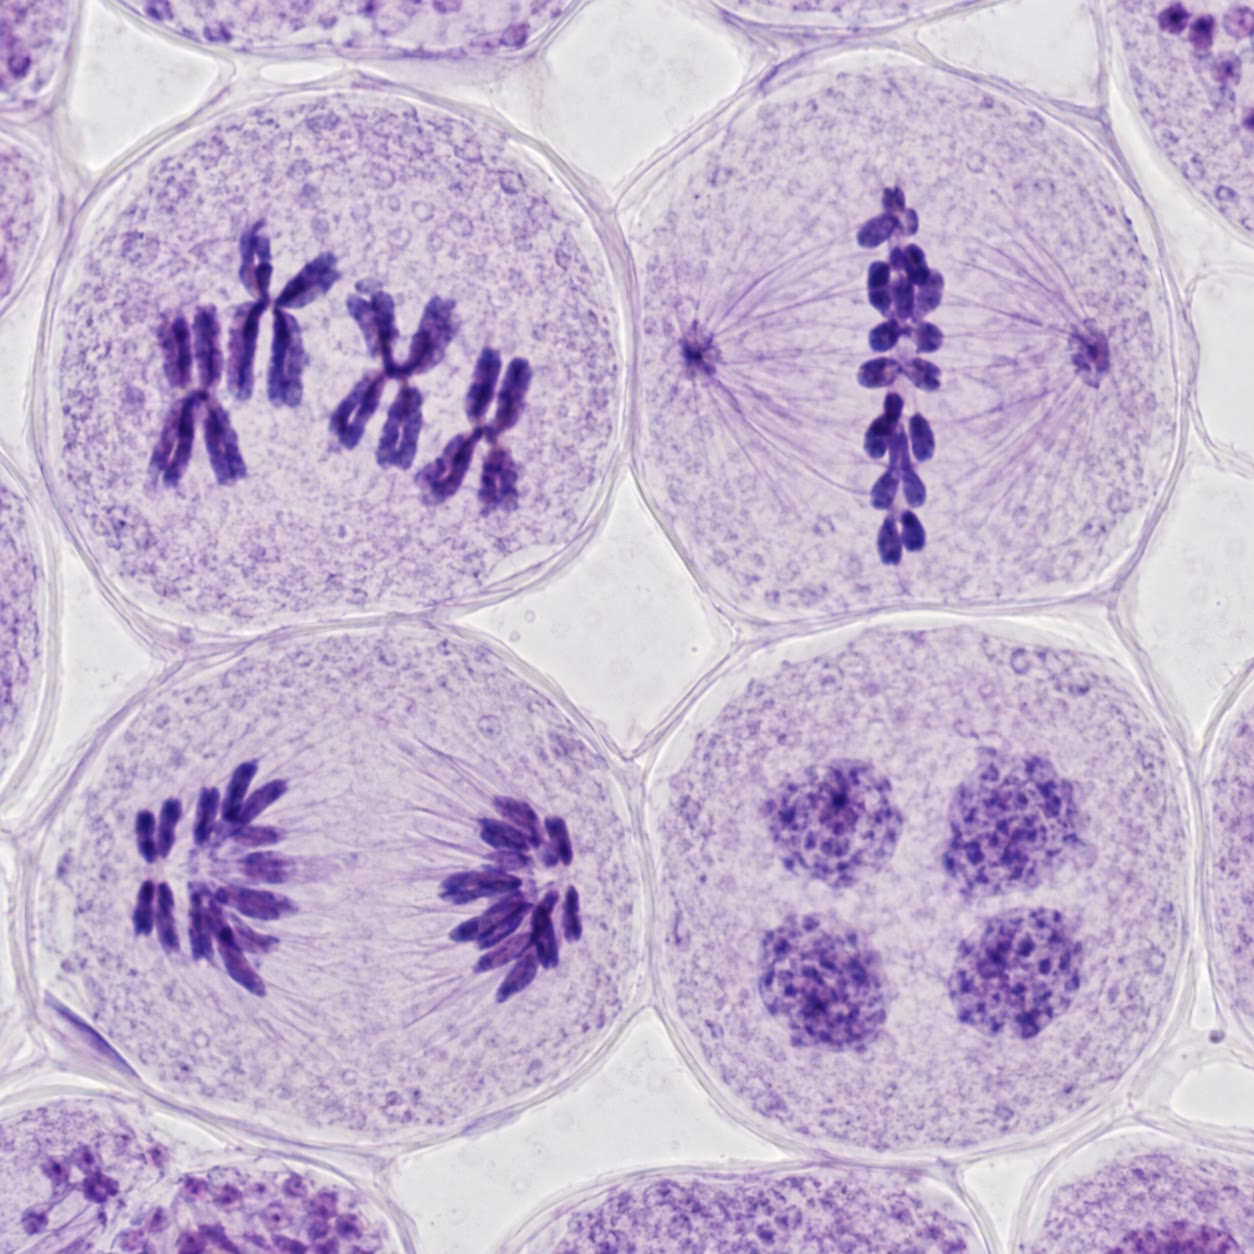
\includegraphics[width=0.5\linewidth]{images/book4/ai/b4-04-lily-meiosis.jpg}

{\small \omterm{def:b2:meiosis-heredity:meiosis}{Meiose} in de helmknop van een lelie: bivalenten in late \omterm{prop:b2:meiosis-heredity:stages}{profase
I}, een metafaseplaat I, anafase I, en de vier kernen van een tetrade.}
\end{omfigure}

\begin{theorem}[Hoeveel menging de meiose oplevert]\label{thm:b2:meiosis-heredity:mixing}
\index{onafhankelijke verdeling}\index{genetische recombinatie}
Voor een organisme met $n$ chromosoomparen levert de willekeurige
oriëntatie van de bivalenten in metafase I $2^n$ mogelijke
combinaties van maternale en paternale chromosomen in een gameet op ---
$2^{23} \approx 8.4$ miljoen bij een mens --- en $2^{2n}$ in een
zygote. Crossing-over vermenigvuldigt dit nog: met ongeveer $k$ chiasmata
per bivalent, elk op een variabele positie, is het aantal verschillende
gameten in feite onbegrensd, en zijn geen twee gameten van één persoon
ooit gelijk. \emph{Recombinatie} --- nieuwe combinaties van \omterm{def:b2:meiosis-heredity:vocabulary}{allelen} ---
ontstaat uit beide: de \omterm{thm:b2:meiosis-heredity:mixing}{onafhankelijke verdeling} husselt hele chromosomen,
crossing-over husselt genen binnen een chromosoom.
\end{theorem}
\begin{proof}
Elk bivalent oriënteert zich onafhankelijk met twee uitkomsten, zodat $n$
bivalenten $2^n$ combinaties geven, alle even waarschijnlijk. Elk van de
twee ouders levert zo'n gameet, zodat de zygote er $2^n\times
2^n$ heeft. Een crossing-over op een bepaalde positie in een chromosoom van $L$
basenparen kan per bivalent in de orde van $L$ verschillende recombinante
chromatiden opleveren, zodat het aantal verschillende producten per
chromosoom groeit als $L^k$, wat astronomisch is voor $L \sim 10^8$.
\end{proof}
\begin{proof}[Bewijsmateriaal]
Creighton en McClintock (1931) gebruikten een chromosoom 9 van maïs dat
twee zichtbare cytologische merkers droeg (een knobbel aan het ene eind,
een getransloceerd segment aan het andere) en daartussen twee genen
(gekleurde/kleurloze korrel, wasachtig/zetmeelrijk endosperm). Onder de
nakomelingen had elke plant met een gerecombineerd paar \omterm{def:b2:meiosis-heredity:vocabulary}{allelen} ook een
gerecombineerd paar cytologische merkers --- knobbel zonder translocatie
of omgekeerd ---, wat bewees dat \omterm{thm:b2:meiosis-heredity:mixing}{genetische recombinatie} een fysieke
uitwisseling van chromosoomsegmenten is.
\end{proof}

\begin{omfigure}
\begin{tikzpicture}[every node/.style={font=\scriptsize}]
  \foreach \dx/\lab/\ca/\cb/\gam in {0/{oriëntatie 1}/omDef/omThm/{gameten AB en ab}, 6.2/{oriëntatie 2}/omThm/omDef/{gameten Ab en aB}} {
    \begin{scope}[xshift=\dx cm]
      \draw[gray, dashed] (0,-1.1) -- (3.2,-1.1);
      \node[anchor=south] at (1.6,0.6) {\lab};
      % pair 1 (long): A above the plate, a below
      \draw[very thick, omDef] (0.7,-0.95) -- (0.7,-0.25); \node[omDef, anchor=south] at (0.7,-0.2) {A};
      \draw[very thick, omThm] (0.7,-1.25) -- (0.7,-1.95); \node[omThm, anchor=north] at (0.7,-2.0) {a};
      % pair 2 (short): B or b above depending on orientation
      \draw[very thick, \ca] (2.3,-0.85) -- (2.3,-0.35);
      \draw[very thick, \cb] (2.3,-1.35) -- (2.3,-1.85);
      \node[anchor=north] at (1.6,-2.4) {\gam};
    \end{scope}
  }
  \node[omDef, anchor=south] at (2.3,-0.3) {B}; \node[omThm, anchor=north] at (2.3,-1.9) {b};
  \node[omThm, anchor=south] at (8.5,-0.3) {b}; \node[omDef, anchor=north] at (8.5,-1.9) {B};
  \node[anchor=north, align=center] at (4.7,-3.0) {elke oriëntatie even waarschijnlijk:\\gameten AB, ab, Ab, aB in gelijke aantallen --- onafhankelijke verdeling};
\end{tikzpicture}

{\small \omterm{thm:b2:meiosis-heredity:mixing}{Onafhankelijke verdeling}. Voor twee chromosoomparen (A/a op het
ene, B/b op het andere) zijn de twee mogelijke oriëntaties van de
bivalenten in metafase I even waarschijnlijk, zodat de vier
allelcombinaties in gelijke aantallen onder de gameten voorkomen.}
\end{omfigure}

\section{Mendeliaanse analyse}

\begin{definition}[Het vocabulaire van kruisingen]\label{def:b2:meiosis-heredity:vocabulary}
\index{allel}\index{genotype}\index{fenotype}\index{dominant}\index{recessief}\index{homozygoot}\index{heterozygoot}
Een \emph{gen} is een stuk chromosoom; zijn \emph{allelen} zijn zijn
sequentievarianten; de \emph{locus} is zijn positie. Een \omterm{def:b2:meiosis-heredity:meiosis}{diploïd}
individu draagt op elke locus twee allelen: zijn \emph{genotype}
is \emph{homozygoot} ($AA$, $aa$) of \emph{heterozygoot} ($Aa$).
Het \emph{fenotype} is het waarneembare kenmerk. Een allel is
\emph{dominant} wanneer de heterozygoot zijn fenotype vertoont,
\emph{recessief} wanneer het alleen bij de homozygoot tot uiting komt;
het onderscheid is een eigenschap van het paar allelen en van het
waargenomen kenmerk, niet van het allel alleen --- de meeste recessieve
allelen zijn functieverliesallelen, verborgen omdat één werkende kopie
volstaat. Een \emph{zuivere lijn} is raszuiver (homozygoot); een
\emph{testkruising} kruist een individu met het dominante fenotype met
een recessieve homozygoot, zodat zijn nakomelingen de allelen van zijn
gameten rechtstreeks onthullen.
\end{definition}

\begin{theorem}[De verhoudingen van Mendel]\label{thm:b2:meiosis-heredity:mendel}
\index{wetten van Mendel}\index{monohybride kruising}\index{dihybride kruising}
Omdat de twee \omterm{def:b2:meiosis-heredity:vocabulary}{allelen} van een \omterm{def:b2:meiosis-heredity:vocabulary}{heterozygoot} $Aa$ in gelijke aantallen
naar verschillende gameten gaan (anafase I), geeft een \emph{monohybride}
kruising $Aa \times Aa$ de \omterm{def:b2:meiosis-heredity:vocabulary}{genotypen} $\tfrac14 AA : \tfrac12 Aa :
\tfrac14 aa$, en de \omterm{def:b2:meiosis-heredity:vocabulary}{fenotypen} $3 : 1$ als $A$ \omterm{def:b2:meiosis-heredity:vocabulary}{dominant} is; de testkruising
$Aa \times aa$ geeft $1 : 1$. Omdat \omterm{def:b2:meiosis-heredity:vocabulary}{allelen} van genen op verschillende
chromosomen onafhankelijk worden verdeeld (metafase I), maakt een
\emph{dihybride}
$AaBb$ vier soorten gameten in gelijke aantallen en geeft de kruising
$AaBb \times AaBb$ de \omterm{def:b2:meiosis-heredity:vocabulary}{fenotypen} $9 : 3 : 3 : 1$, de testkruising
$AaBb \times aabb$ geeft $1 : 1 : 1 : 1$. Voor $k$ onafhankelijke
heterozygote loci is het aantal gameettypen $2^k$ en is de
fenotypische verhouding het product van $k$ verhoudingen $3 : 1$.
\end{theorem}
\begin{proof}
Segregatie: de gameten van de \omterm{def:b2:meiosis-heredity:vocabulary}{heterozygoot} zijn $\tfrac12 A$,
$\tfrac12 a$; bij willekeurige bevruchting zijn de \omterm{def:b2:meiosis-heredity:vocabulary}{genotypen} van de zygote de
producten $(\tfrac12 A + \tfrac12 a)^2 = \tfrac14 AA + \tfrac12 Aa +
\tfrac14 aa$. Onafhankelijkheid: de gameten van $AaBb$ zijn $(\tfrac12 A
+ \tfrac12 a)(\tfrac12 B + \tfrac12 b)$, vier soorten met elk $\tfrac14$;
de dihybride \omterm{def:b2:meiosis-heredity:vocabulary}{fenotypen} vermenigvuldigen $(\tfrac34 A\_ + \tfrac14 aa)
(\tfrac34 B\_ + \tfrac14 bb)$, wat $\tfrac{9}{16}, \tfrac{3}{16},
\tfrac{3}{16}, \tfrac{1}{16}$ geeft. Elke factor is één onafhankelijke
segregatie, zodat $k$ loci een product van $k$ factoren geven.
\end{proof}
\begin{proof}[Bewijsmateriaal]
Mendel (1866) kruiste zuivere lijnen van erwt die in één kenmerk
verschilden --- ronde of gerimpelde zaden, gele of groene zaadlobben,
paarse of witte bloemen, hoge of dwergstengels en nog drie andere --- en
vond in elk geval een uniforme eerste generatie en een tweede generatie
die dicht bij $3 : 1$ uitsplitste: 5474 rond tegen 1850 gerimpeld ($2.96 :
1$), 6022 geel tegen 2001 groen ($3.01 : 1$), 705 paars tegen 224 wit
($3.15 : 1$). Bij kruisingen met twee kenmerken vond hij $315 : 108 : 101 :
32$ ($9 : 3 : 3 : 1$), en door de tweede generatie verder te kweken
toonde hij aan dat de dominante klasse uit twee soorten bestond, een derde
raszuiver en twee derde uitsplitsend. De chromosomen die de verhoudingen
verklaren, werden veertig jaar later gevonden.
\end{proof}

\begin{omfigure}
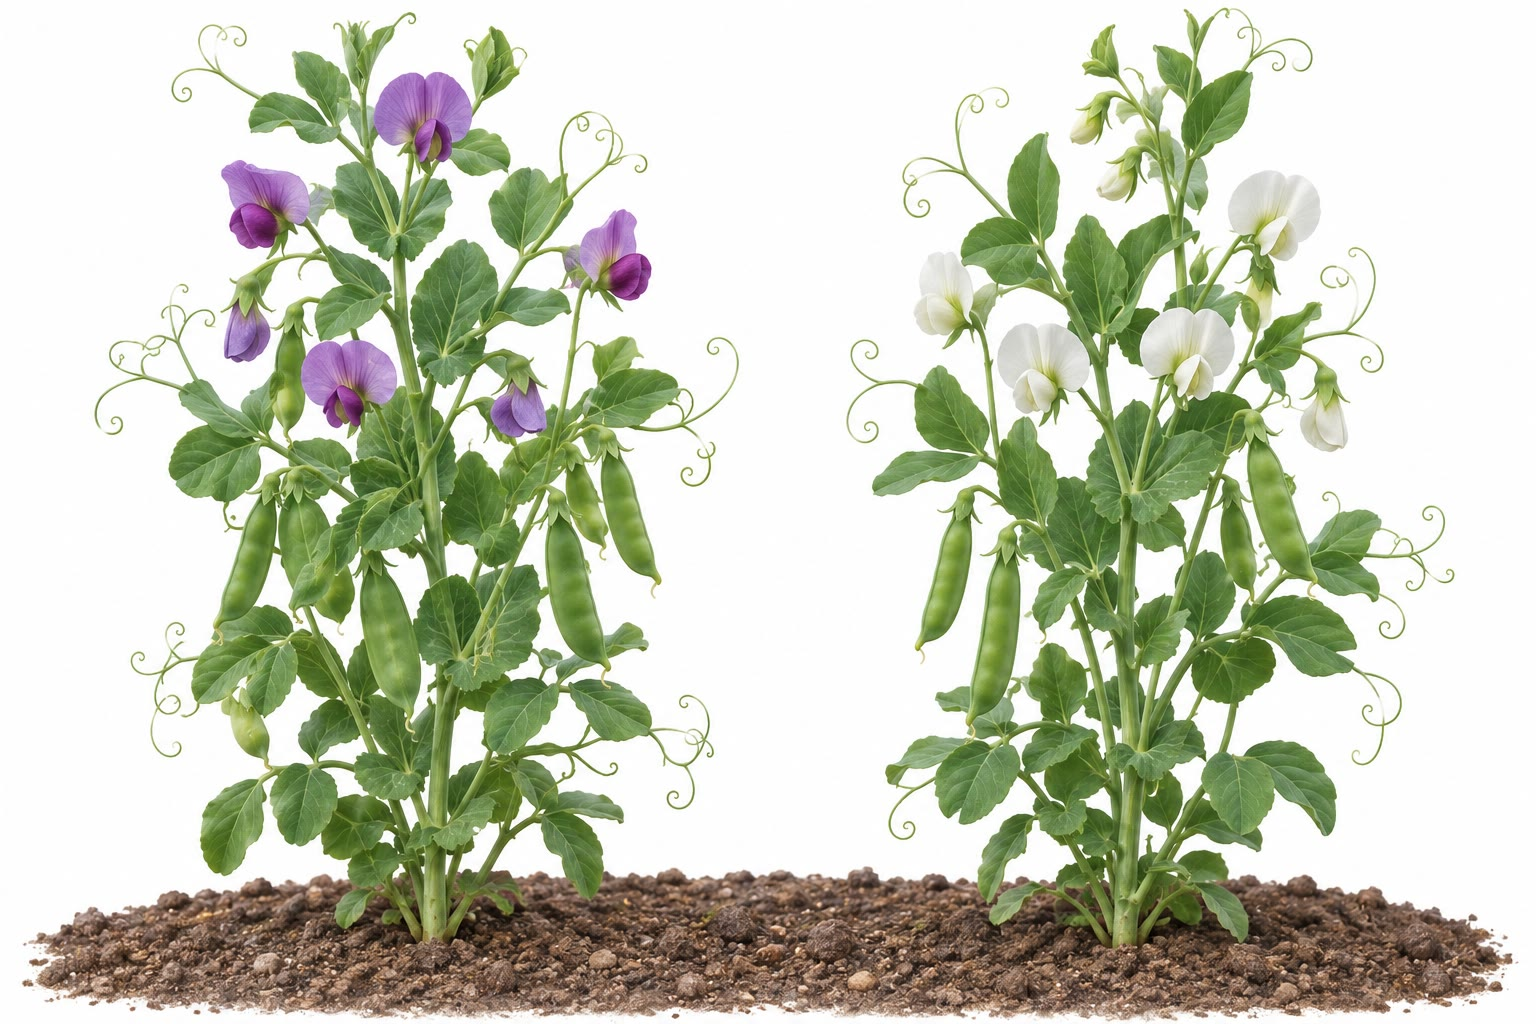
\includegraphics[width=0.58\linewidth]{images/book4/ai/b4-04-pea-flowers.jpg}

{\small Erwtenplanten met paarse en met witte bloemen: een van de zeven
kenmerkparen waarop Mendel de genetica grondvestte. De hybride met paarse
bloemen geeft na zelfbestuiving ongeveer drie paarse op één witte.}
\end{omfigure}

\begin{method}[Een verhouding toetsen met $\chi^2$]\label{met:b2:meiosis-heredity:chisquare}
\index{chikwadraattoets}
Om te beslissen of waargenomen aantallen $O_i$ bij een veronderstelde verhouding passen:
\begin{enumerate}
  \item Bereken de verwachte aantallen $E_i$ uit de verhouding en het
        totaal.
  \item Bereken $\chi^2 = \sum_i (O_i - E_i)^2/E_i$.
  \item Tel de vrijheidsgraden: het aantal klassen min
        één.
  \item Vergelijk met de kritische waarde op het \qty{5}{\%}-niveau:
        $3.84$ bij 1 vrijheidsgraad, $5.99$ bij 2, $7.81$ bij 3,
        $9.49$ bij 4. Ligt $\chi^2$ eronder, dan zijn de gegevens
        verenigbaar met de verhouding; ligt het erboven, dan wordt de
        verhouding verworpen --- de afwijking zou dan in minder dan één
        experiment op twintig door toeval ontstaan.
\end{enumerate}
Voor de bloemen van Mendel, $705 : 224$ tegen $3 : 1$: $E = 696.75,
232.25$; $\chi^2 = 0.098 + 0.293 = 0.39 < 3.84$. (De verdeling
achter de kritische waarden wordt afgeleid in de statistiek van de
wiskundereeks; hier is de tabel een hulpmiddel.)
\end{method}

\begin{proposition}[Voorbij de eenvoudige verhoudingen]\label{prop:b2:meiosis-heredity:extensions}
\index{onvolledige dominantie}\index{codominantie}\index{epistasie}\index{letaal allel}
De verhoudingen veranderen, maar het mechanisme niet, wanneer: \omterm{def:b2:meiosis-heredity:vocabulary}{allelen}
\emph{\omterm{prop:b2:meiosis-heredity:extensions}{onvolledige dominantie}} vertonen (rode $\times$ witte leeuwenbek
geeft roze, en de tweede generatie $1 : 2 : 1$); \omterm{def:b2:meiosis-heredity:vocabulary}{allelen}
\emph{codominant} zijn en beide tot uiting komen (bloedgroep $AB$: de
\omterm{def:b2:meiosis-heredity:vocabulary}{heterozygoot} $I^AI^B$ maakt beide antigenen; een locus kan \emph{meerdere
\omterm{def:b2:meiosis-heredity:vocabulary}{allelen}} hebben, $I^A$, $I^B$, $i$); een \omterm{def:b2:meiosis-heredity:vocabulary}{allel} \emph{letaal} is in
homozygote toestand (gele muizen: geel $\times$ geel geeft $2$ geel op
$1$ agouti, omdat de $\tfrac14 YY$ als embryo sterven); twee genen in
één route werken (\emph{epistasie}: in een kruising $9 : 3 : 3 : 1$
kunnen de dubbel recessieve en één enkelvoudig recessieve klasse niet te
onderscheiden zijn, wat
$9 : 3 : 4$ geeft, zoals bij albinomuizen, of kunnen beide dominante
\omterm{def:b2:meiosis-heredity:vocabulary}{allelen} nodig zijn voor het \omterm{def:b2:meiosis-heredity:vocabulary}{fenotype}, wat $9 : 7$ geeft, zoals bij paarse
lathyrussen die twee enzymen nodig hebben om hun pigment te maken); veel
genen elk een beetje bijdragen aan een continu kenmerk (lengte,
opbrengst), wat de kwantitatieve genetica is van
\cref{ch:b2:population-genetics}. Een verhouding terugvoeren op een
mechanisme is het dagelijkse ambacht van de genetica.
\end{proposition}

\section{Koppeling en genetische kaarten}

\begin{definition}[Koppeling en recombinatiefrequentie]\label{def:b2:meiosis-heredity:linkage}
\index{koppeling}\index{recombinatiefrequentie}\index{centimorgan}
Twee genen op hetzelfde chromosoom zijn \emph{gekoppeld}: hun \omterm{def:b2:meiosis-heredity:vocabulary}{allelen}
gaan bij voorkeur samen naar de gameten, en een dihybride
$AB/ab$ maakt meer \emph{parentale} gameten ($AB$, $ab$) dan
\emph{recombinante} ($Ab$, $aB$). Recombinanten ontstaan alleen wanneer
een crossing-over tussen de twee loci valt, zodat hun frequentie $r$ ---
rechtstreeks geteld in een testkruising --- de afstand meet: $r$
loopt van 0 (volledige koppeling) tot $\tfrac12$ (genen die zo ver uit
elkaar liggen, of op verschillende chromosomen, dat ze onafhankelijk
worden verdeeld). De eenheid van \emph{kaartafstand} is de
\emph{centimorgan} (cM): \qty{1}{cM}
is \qty{1}{\%} recombinatie voor nauw gekoppelde genen; bij de mens
is \qty{1}{cM} ongeveer een miljoen basenparen. Koppeling was het eerste
bewijs dat genen op een rij op het chromosoom liggen.
\end{definition}
\begin{proof}[Bewijsmateriaal]
Morgan (1911) vond dat de genen voor witte ogen en miniatuurvleugels van
de fruitvlieg, beide op het X-chromosoom, niet onafhankelijk werden
verdeeld: een testkruising gaf \qty{37}{\%} recombinanten in plaats van
\qty{50}{\%}, en andere paren gaven andere, reproduceerbare percentages.
Sturtevant (1913), toen nog student, besefte dat als de frequenties
afstanden meten, ze optelbaar moeten zijn: uit de paarsgewijze
frequenties van zes X-gebonden genen tekende hij de eerste genetische
kaart, en de afstanden waren, binnen de meetfout, optelbaar langs een lijn.
\end{proof}

\begin{omfigure}
\begin{tikzpicture}[every node/.style={font=\scriptsize}]
  % bivalent with crossover between A and B
  \draw[very thick, omDef] (0,1.2) -- (2.0,1.2) -- (3.0,0.6) -- (5,0.6);
  \draw[very thick, omDef] (0,1.5) -- (5,1.5);
  \draw[very thick, omThm] (0,0.3) -- (2.0,0.3) -- (3.0,0.9) -- (5,0.9);
  \draw[very thick, omThm] (0,0) -- (5,0);
  \node[omDef, above] at (0.8,1.5) {A}; \node[omDef, above] at (4.3,1.5) {B};
  \node[omThm, below] at (0.8,0) {a}; \node[omThm, below] at (4.3,0) {b};
  \node[anchor=south, gray] at (2.5,1.85) {crossing-over tussen de loci A en B};
  % products
  \draw[->, thick, gray] (5.4,0.75) -- (6.2,0.75);
  \node[anchor=west, align=left] at (6.4,1.45) {\textcolor{omDef}{A\,B} \quad parentaal};
  \node[anchor=west, align=left] at (6.4,0.95) {\textcolor{omDef}{A}\,\textcolor{omThm}{b} \quad recombinant};
  \node[anchor=west, align=left] at (6.4,0.5) {\textcolor{omThm}{a}\,\textcolor{omDef}{B} \quad recombinant};
  \node[anchor=west, align=left] at (6.4,0.0) {\textcolor{omThm}{a\,b} \quad parentaal};
  \node[anchor=west, align=left, text width=5.6cm] at (6.4,-0.9) {één crossing-over tussen de loci in een fractie $c$ van de meiosen: recombinante gameten $r = c/2$, omdat maar twee van de vier chromatiden worden uitgewisseld};
\end{tikzpicture}

{\small Recombinatie tussen twee gekoppelde loci. Een crossing-over
tussen beide in een bivalent wisselt de \omterm{def:b2:meiosis-heredity:vocabulary}{allelen} op twee van de vier
chromatiden uit; de recombinante gameten worden in een testkruising
geteld, en hun frequentie meet de afstand.}
\end{omfigure}

\begin{method}[Twee gekoppelde genen in kaart brengen]\label{met:b2:meiosis-heredity:twopoint}
\begin{enumerate}
  \item Kruis twee zuivere lijnen om de dihybride te verkrijgen; noteer
        welke \omterm{def:b2:meiosis-heredity:vocabulary}{allelen} hij samen ontving (zijn parentale combinaties,
        \emph{koppelingsfase} $AB/ab$ of \emph{afstotingsfase} $Ab/aB$).
  \item Kruis hem terug met de dubbel recessieve en deel de
        nakomelingen in: de twee talrijkste klassen zijn parentaal, de
        twee minst talrijke recombinant.
  \item $r = $ recombinanten $/$ totaal; de afstand is $100\,r$ cM.
  \item Controleer eerst de onafhankelijkheid: zijn de vier klassen gelijk
        ($\chi^2$ tegen $1 : 1 : 1 : 1$), dan zijn de genen niet gekoppeld.
\end{enumerate}
\end{method}

\begin{theorem}[De karteringsfunctie van Haldane]\label{thm:b2:meiosis-heredity:haldane}
\index{karteringsfunctie}
De \omterm{def:b2:meiosis-heredity:linkage}{recombinatiefrequentie} onderschat de afstand voor ver uit elkaar
liggende genen, omdat twee crossing-overs ertussen de parentale
combinatie herstellen. Als crossing-overs onafhankelijk langs het
chromosoom vallen (geen interferentie), met $d$ de kaartafstand in morgan
(verwacht aantal crossing-overs per chromatide), is de recombinatiefractie
\[
r = \tfrac12\,\bigl(1 - e^{-2d}\bigr), \qquad d = -\tfrac12\ln(1 - 2r),
\]
zodat $r \approx d$ voor kleine $d$ en $r \to \tfrac12$ naarmate $d$
groeit; $r = 0.40$ komt overeen met \qty{80}{cM}, en \qty{50}{cM}
geeft $r = 0.32$. Echte chromosomen vertonen \emph{interferentie} --- een
crossing-over maakt een andere in de buurt minder waarschijnlijk --- wat
$r$ over korte afstanden dichter bij $d$ brengt dan Haldane voorspelt.
\end{theorem}
\begin{proof}
Zij de kaartafstand $d$ het verwachte aantal crossing-overs per
chromatide in het interval; omdat elke crossing-over twee van de
vier chromatiden betreft, draagt het bivalent als geheel een
poissonverdeeld aantal crossing-overs met gemiddelde $2d$ in het
interval, en is de kans dat het er geen draagt $e^{-2d}$. Draagt het er
minstens één, dan betreft elke crossing-over onafhankelijk een gegeven
chromatide met kans
$\tfrac12$, zodat een gegeven chromatide een oneven aantal keren is
uitgewisseld --- recombinant is --- met kans precies $\tfrac12$,
ongeacht het aantal crossing-overs. Dus $r = \tfrac12\,(1 -
e^{-2d})$; omkeren geeft $d$. Voor kleine $d$ is $r \approx d$; voor
$d \to \infty$ gaat $r \to \tfrac12$.
\end{proof}

\begin{omfigure}
\begin{tikzpicture}
\begin{axis}[
  width=0.72\linewidth, height=5.6cm,
  axis x line=bottom, axis y line=left,
  xmin=0, xmax=150, ymin=0, ymax=0.55,
  xlabel={kaartafstand $d$ (cM)}, ylabel={recombinatiefractie $r$},
  xlabel style={font=\small, at={(axis description cs:0.5,-0.13)}, anchor=north},
  ylabel style={font=\small},
  tick label style={font=\small}, xtick={0,50,100,150}, ytick={0,0.25,0.5},
  legend style={font=\scriptsize, at={(0.97,0.1)}, anchor=south east, draw=none},
  clip=false,
]
\addplot[very thick, omDef, domain=0:150, samples=80] {0.5*(1-exp(-2*x/100))};
\addlegendentry{Haldane: $r = \tfrac12(1 - e^{-2d})$}
\addplot[thick, dashed, gray, domain=0:50, samples=2] {x/100};
\addlegendentry{$r = d$ (geen dubbele crossing-overs)}
\draw[dashed, gray] (axis cs:0,0.5) -- (axis cs:150,0.5);
\end{axis}
\end{tikzpicture}

{\small Recombinatiefractie tegen kaartafstand. Nabije genen recombineren
naar verhouding van hun afstand; verre genen komen nooit boven
\qty{50}{\%} recombinatie, hoe ver ze ook uit elkaar liggen, omdat dubbele
crossing-overs de parentale combinaties herstellen.}
\end{omfigure}

\begin{method}[De driepuntstestkruising]\label{met:b2:meiosis-heredity:threepoint}
\index{driepuntskruising}\index{interferentie}
Kruis een drievoudige \omterm{def:b2:meiosis-heredity:vocabulary}{heterozygoot} $ABC/abc$ met $abc/abc$ en deel de
acht klassen van nakomelingen in.
\begin{enumerate}
  \item De twee grootste klassen zijn de parentale; de twee kleinste
        zijn de \emph{dubbele crossing-overs}.
  \item Het gen dat wisselt tussen een parentale klasse en de klasse van
        de dubbele crossing-over, is het \emph{middelste}: dit geeft
        de volgorde.
  \item Voor elk aangrenzend paar is de \omterm{def:b2:meiosis-heredity:linkage}{recombinatiefrequentie}
        (enkele crossing-overs in dat interval + dubbele crossing-overs) $/$
        totaal, omdat een dubbele crossing-over beide intervallen recombineert.
  \item Verwachte dubbele crossing-overs $= r_1 r_2 \times$ totaal; de
        \emph{coïncidentiecoëfficiënt} is waargenomen/verwacht en
        de \emph{interferentie} is $1 -$ coïncidentie.
\end{enumerate}
\end{method}

\begin{example}[Een uitgewerkte driepuntskruising]\label{ex:b2:meiosis-heredity:threepoint}
Nakomelingen van $+++/abc \times abc/abc$: $+++$ 580, $abc$ 592, $++c$
45, $ab+$ 40, $+bc$ 89, $a++$ 94, $+b+$ 3, $a+c$ 5; totaal 1448.
Parentaal $+++$, $abc$; dubbel $+b+$, $a+c$; vergelijking van $+++$ met
$+b+$ toont dat het gewisselde gen $b$ is: volgorde $a$--$b$--$c$. $r_{ab} =
(89 + 94 + 3 + 5)/1448 = 0.132$; $r_{bc} = (45 + 40 + 3 + 5)/1448 =
0.064$; kaart: $a$ --- \qty{13.2}{cM} --- $b$ --- \qty{6.4}{cM} ---
$c$. Verwachte dubbele $0.132\times 0.064\times 1448 = 12.2$,
waargenomen 8: coïncidentie $0.65$, interferentie $0.35$.
\end{example}

\begin{omfigure}
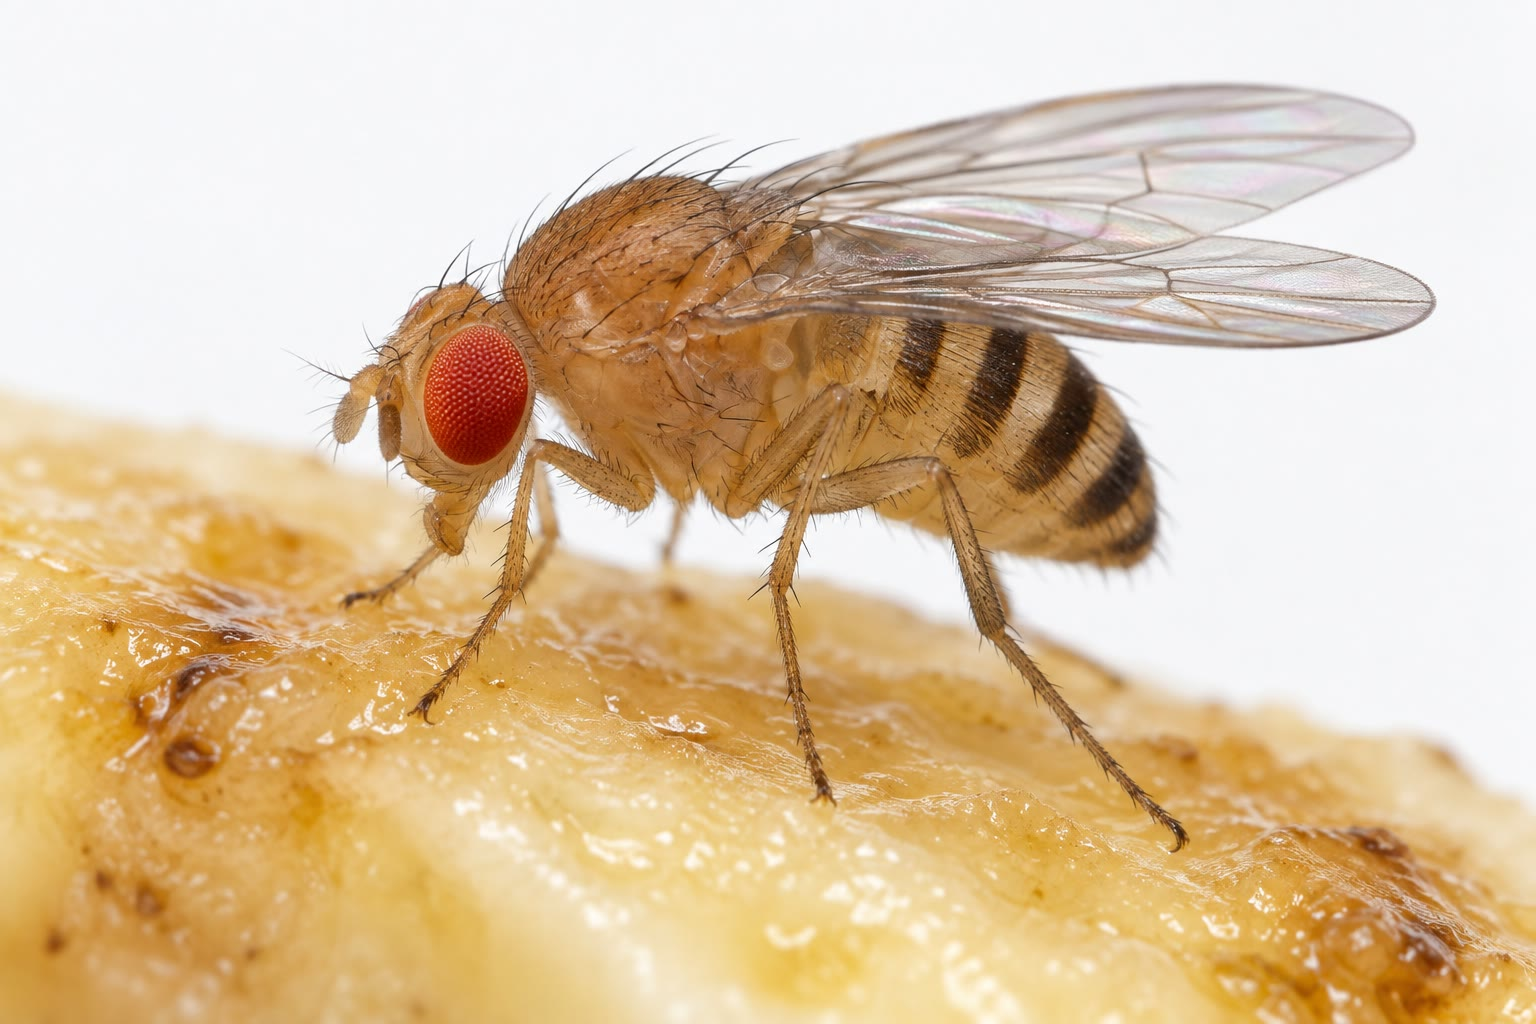
\includegraphics[width=0.5\linewidth]{images/book4/ai/b4-04-drosophila.jpg}

{\small \emph{Drosophila melanogaster}: twee weken per generatie,
honderden nakomelingen, vier chromosoomparen en een eeuw aan mutanten ---
het organisme waarop \omterm{def:b2:meiosis-heredity:linkage}{koppeling}, kaarten en geslachtsgebonden overerving
werden uitgewerkt.}
\end{omfigure}

\section{Geslachtschromosomen en organellen}

\begin{proposition}[Geslachtsgebonden overerving]\label{prop:b2:meiosis-heredity:sexlinked}
\index{X-gebonden overerving}\index{geslachtschromosomen}
Bij zoogdieren en vliegen is het vrouwtje $XX$ en het mannetje $XY$: de $Y$
draagt weinig genen, zodat een mannetje van elk $X$-gebonden gen één
enkele kopie heeft (hij is \emph{hemizygoot}) en elk \omterm{def:b2:meiosis-heredity:vocabulary}{allel} dat hij draagt
tot uiting brengt, \omterm{def:b2:meiosis-heredity:vocabulary}{dominant} of \omterm{def:b2:meiosis-heredity:vocabulary}{recessief}. Gevolgen: reciproke kruisingen
verschillen (vrouwtje met witte ogen $\times$ mannetje met rode ogen geeft
zonen met witte ogen en dochters met rode ogen; de omgekeerde kruising
geeft alleen rode); een \omterm{def:b2:meiosis-heredity:vocabulary}{recessief} $X$-gebonden kenmerk (rood-groenkleurenblindheid,
hemofilie, spierdystrofie van Duchenne) komt vooral bij mannen voor, wordt
doorgegeven door niet-aangedane draagsters, en wordt nooit van vader op
zoon doorgegeven (een zoon krijgt de $Y$ van zijn vader); een vader geeft
zijn $X$ aan al zijn dochters. Vogels, vlinders en sommige reptielen
keren de regeling om ($ZW$-vrouwtjes, $ZZ$-mannetjes); bij veel reptielen
beslist de temperatuur; en bij zoogdieren wordt in elke vrouwelijke cel
vroeg in de ontwikkeling willekeurig één $X$ uitgeschakeld, zodat een
\omterm{def:b2:meiosis-heredity:vocabulary}{heterozygoot} vrouwtje een mozaïek is (de lapjeskat).
\end{proposition}
\begin{proof}[Bewijsmateriaal]
Morgan (1910) vond één mannetje met witte ogen tussen duizenden
roodogige vliegen. Gekruist met rode vrouwtjes waren alle nakomelingen
rood; maar in de volgende generatie verschenen de witte ogen alleen bij
mannetjes terug, bij de helft van hen. Een kruising van een wit mannetje
met zijn rode dochters gaf witte ogen bij beide geslachten. Het patroon
was precies wat men verwacht als het gen op het X-chromosoom lag, dat
vrouwtjes twee keer en mannetjes één keer dragen --- het eerste gen dat
aan een chromosoom werd toegewezen.
\end{proof}

\begin{omfigure}
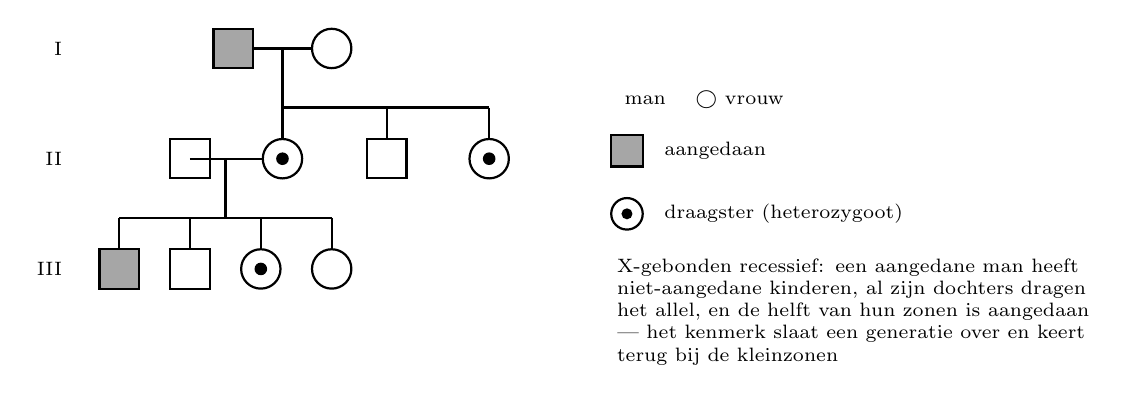
\begin{tikzpicture}[every node/.style={font=\scriptsize}]
  % pedigree: X-linked recessive
  \draw[thick, fill=gray!70] (0,0) rectangle (0.5,0.5); % affected grandfather
  \draw[thick] (1.5,0.25) circle (0.25);
  \draw[thick] (0.5,0.25) -- (1.25,0.25);
  \draw[thick] (0.875,0.25) -- (0.875,-0.5);
  \draw[thick] (0.875,-0.5) -- (3.5,-0.5);
  % children of generation I
  \draw[thick] (0.875,-0.5) -- (0.875,-0.9); \draw[thick, fill=white] (0.875,-1.15) circle (0.25); \fill (0.875,-1.15) circle (0.08);
  \draw[thick] (2.2,-0.5) -- (2.2,-0.9); \draw[thick] (1.95,-1.4) rectangle (2.45,-0.9);
  \draw[thick] (3.5,-0.5) -- (3.5,-0.9); \draw[thick, fill=white] (3.5,-1.15) circle (0.25); \fill (3.5,-1.15) circle (0.08);
  % carrier daughter marries
  \draw[thick] (-0.3,-1.15) -- (0.625,-1.15); \draw[thick] (-0.55,-1.4) rectangle (-0.05,-0.9);
  \draw[thick] (0.15,-1.15) -- (0.15,-1.9); \draw[thick] (-1.2,-1.9) -- (1.5,-1.9);
  \draw[thick] (-1.2,-1.9) -- (-1.2,-2.3); \draw[thick, fill=gray!70] (-1.45,-2.8) rectangle (-0.95,-2.3);
  \draw[thick] (-0.3,-1.9) -- (-0.3,-2.3); \draw[thick] (-0.55,-2.8) rectangle (-0.05,-2.3);
  \draw[thick] (0.6,-1.9) -- (0.6,-2.3); \draw[thick, fill=white] (0.6,-2.55) circle (0.25); \fill (0.6,-2.55) circle (0.08);
  \draw[thick] (1.5,-1.9) -- (1.5,-2.3); \draw[thick, fill=white] (1.5,-2.55) circle (0.25);
  \node[anchor=east] at (-1.8,0.25) {I};
  \node[anchor=east] at (-1.8,-1.15) {II};
  \node[anchor=east] at (-1.8,-2.55) {III};
  % legend
  \node[anchor=west, align=left] at (5,-0.4) {$\square$ man \quad $\bigcirc$ vrouw};
  \draw[thick, fill=gray!70] (5.05,-1.25) rectangle (5.45,-0.85); \node[anchor=west] at (5.6,-1.05) {aangedaan};
  \draw[thick] (5.25,-1.85) circle (0.2); \fill (5.25,-1.85) circle (0.07); \node[anchor=west] at (5.6,-1.85) {draagster (heterozygoot)};
  \node[anchor=north west, align=left, text width=6.2cm] at (5,-2.3) {X-gebonden recessief: een aangedane man heeft niet-aangedane kinderen, al zijn dochters dragen het allel, en de helft van hun zonen is aangedaan --- het kenmerk slaat een generatie over en keert terug bij de kleinzonen};
\end{tikzpicture}

{\small Een stamboom van een X-gebonden \omterm{def:b2:meiosis-heredity:vocabulary}{recessief} kenmerk zoals
hemofilie: geen overdracht van vader op zoon, dochters die draagster zijn,
aangedane kleinzonen.}
\end{omfigure}

\begin{method}[Een stamboom lezen]\label{met:b2:meiosis-heredity:pedigree}
\index{stamboom}
\begin{enumerate}
  \item Twee niet-aangedane ouders met een aangedaan kind: het kenmerk is
        \omterm{def:b2:meiosis-heredity:vocabulary}{recessief} (beide ouders \omterm{def:b2:meiosis-heredity:vocabulary}{heterozygoot}).
  \item Een aangedaan kind heeft altijd een aangedane ouder, en het
        kenmerk komt in elke generatie voor: \omterm{def:b2:meiosis-heredity:vocabulary}{dominant}.
  \item Aangedane individuen vooral mannelijk, doorgegeven via
        niet-aangedane moeders, nooit van vader op zoon: X-gebonden \omterm{def:b2:meiosis-heredity:vocabulary}{recessief}.
  \item Een aangedane vader heeft alleen aangedane dochters en geen
        aangedane zoon: X-gebonden \omterm{def:b2:meiosis-heredity:vocabulary}{dominant}.
  \item Door moeders aan al hun kinderen doorgegeven, nooit door
        vaders: mitochondriaal.
  \item Bereken daarna kansen uit de afgeleide \omterm{def:b2:meiosis-heredity:vocabulary}{genotypen}:
        een koppel draagster $\times$ normaal heeft bij elke geboorte een kans
        van $\tfrac14$ op een aangedane zoon ($\tfrac12$ jongen $\times$ $\tfrac12$
        ontvangt het \omterm{def:b2:meiosis-heredity:vocabulary}{allel}).
\end{enumerate}
\end{method}

\begin{definition}[Extranucleaire overerving]\label{def:b2:meiosis-heredity:extranuclear}
\index{maternale overerving}\index{mitochondriale overerving}
Mitochondriën en chloroplasten dragen hun eigen kleine genomen, in vele
kopieën per organel en met vele organellen per cel, en ze komen vrijwel
volledig uit de eicel: de zaadcel levert een kern en weinig meer. Hun
genen worden daarom \emph{maternaal
overgeërfd}, zonder uitsplitsingsverhoudingen: een moeder geeft het
kenmerk door aan al haar kinderen, een vader aan geen enkel. Menselijke
mitochondriale ziekten (defecten van de ademhalingsketen die spieren en
zenuwen treffen) volgen dit patroon, en zo ook de bontbladigheid van
sommige planten, waarbij een moedercel met zowel normale als mutante
chloroplasten die willekeurig over de dochtercellen verdeelt, zodat groene,
witte en gemengde sectoren ontstaan. Omdat ze nooit recombineren, volgen
mitochondriale sequenties maternale lijnen terug in de tijd --- het
instrument van \cref{ch:b2:phylogenetic-trees}.
\end{definition}

\begin{proposition}[Tetradenanalyse]\label{prop:b2:meiosis-heredity:tetrads}
\index{tetradenanalyse}\index{geordende tetrade}
Bij sommige schimmels (\emph{Neurospora}, \emph{Sordaria}) blijven de
vier producten van één \omterm{def:b2:meiosis-heredity:meiosis}{meiose} samen in een zakje, de \emph{ascus}, en wel
in volgorde: een laatste mitose geeft acht sporen waarvan de volgorde de
twee delingen vastlegt. Voor een \omterm{def:b2:meiosis-heredity:vocabulary}{heterozygoot} $A/a$ had een ascus met het
patroon $4 : 4$ (\emph{segregatie bij de eerste deling}) geen
crossing-over tussen het gen en zijn centromeer --- de \omterm{def:b2:meiosis-heredity:vocabulary}{allelen} gingen in
anafase I uiteen; een patroon $2 : 2 : 2 : 2$ of $2 : 4 : 2$
(\emph{segregatie bij de tweede deling}) had er één, zodat de \omterm{def:b2:meiosis-heredity:vocabulary}{allelen} pas
in anafase II uiteengingen. De afstand van gen tot centromeer is de helft
van het percentage asci met segregatie bij de tweede deling, omdat een
crossing-over maar twee van de vier chromatiden recombineert. Tetraden
tonen ook rechtstreeks dat recombinatie wederkerig is: elke recombinante
chromatide heeft haar complementaire partner in dezelfde ascus.
\end{proposition}

\begin{omfigure}
\begin{tikzpicture}[every node/.style={font=\scriptsize}]
  \foreach \dx/\pat/\lab in {0/{omDef,omDef,omDef,omDef,omThm,omThm,omThm,omThm}/{$4:4$, geen crossing-over:\\segregatie bij\\de eerste deling}, 4.5/{omDef,omDef,omThm,omThm,omDef,omDef,omThm,omThm}/{$2:2:2:2$, crossing-over tussen\\gen en centromeer}, 9/{omDef,omDef,omThm,omThm,omThm,omThm,omDef,omDef}/{$2:4:2$, crossing-over:\\segregatie bij\\de tweede deling}} {
    \begin{scope}[xshift=\dx cm]
      \draw[thick, rounded corners=6pt] (0,0) rectangle (0.8,4.2);
      \foreach \c [count=\i] in \pat { \fill[\c] (0.4,4.2-0.5*\i+0.02) circle (0.2); }
      \node[below, align=center] at (0.4,-0.1) {\lab};
    \end{scope}
  }
  \node[anchor=west, align=left, text width=2.6cm] at (12.4,3.2) {geordende asci van \emph{Sordaria}; blauwe en rode sporen dragen de twee allelen};
\end{tikzpicture}

{\small \omterm{prop:b2:meiosis-heredity:tetrads}{Geordende tetraden}. Zonder crossing-over tussen het gen en zijn
centromeer scheiden de \omterm{def:b2:meiosis-heredity:vocabulary}{allelen} bij de eerste deling en lezen de acht
sporen $4 : 4$; met één scheiden ze bij de tweede deling en leest de
ascus $2 : 2 : 2 : 2$ of $2 : 4 : 2$.}
\end{omfigure}

\section{Opgaven}

\begin{exercise}[$\star$]\label{exo:b2:meiosis-heredity:1}
Noem vier verschillen tussen mitose en \omterm{def:b2:meiosis-heredity:meiosis}{meiose} (aantal delingen, paring,
producten, genetische identiteit van de producten).
\end{exercise}

\begin{exercise}[$\star$]\label{exo:b2:meiosis-heredity:2}
Hoeveel chromosomaal verschillende gameten kan een mens maken door
\omterm{thm:b2:meiosis-heredity:mixing}{onafhankelijke verdeling} alleen? Een fruitvlieg ($n = 4$)? Een erwt ($n =
7$)?
\end{exercise}

\begin{exercise}[$\star$]\label{exo:b2:meiosis-heredity:3}
Bij erwten is hoog ($T$) \omterm{def:b2:meiosis-heredity:vocabulary}{dominant} over dwerg. Geef de fenotypische en
genotypische verhoudingen van $Tt \times Tt$ en van $Tt \times tt$. Hoe
ga je na of een hoge plant $TT$ of $Tt$ is?
\end{exercise}

\begin{exercise}[$\star$]\label{exo:b2:meiosis-heredity:4}
Definieer \omterm{def:b2:meiosis-heredity:linkage}{koppeling}, \omterm{def:b2:meiosis-heredity:linkage}{recombinatiefrequentie} en de \omterm{def:b2:meiosis-heredity:linkage}{centimorgan}. Waarom
kunnen twee genen op hetzelfde chromosoom toch worden verdeeld alsof ze
onafhankelijk waren?
\end{exercise}

\begin{exercise}[$\star\star$]\label{exo:b2:meiosis-heredity:5}
De \omterm{thm:b2:meiosis-heredity:mendel}{dihybride kruising} van Mendel gaf $315$ rond geel, $108$ rond groen,
$101$ gerimpeld geel, $32$ gerimpeld groen. Toets de hypothese $9 : 3 : 3 :
1$ met $\chi^2$ (3 vrijheidsgraden, kritische waarde
$7.81$).
\end{exercise}

\begin{exercise}[$\star\star$]\label{exo:b2:meiosis-heredity:6}
Een dihybride $AB/ab$ geeft bij een testkruising $412$ $AB$, $388$ $ab$, $103$
$Ab$, $97$ $aB$. Zijn de genen gekoppeld? Bereken de \omterm{def:b2:meiosis-heredity:linkage}{recombinatiefrequentie}
en de kaartafstand; wat zou de dihybride $Ab/aB$ geven?
\end{exercise}

\begin{exercise}[$\star\star$]\label{exo:b2:meiosis-heredity:7}
Zet met de functie van Haldane $r = 0.20$ en $r = 0.45$ om in
kaartafstanden, en \qty{30}{cM} en \qty{100}{cM} in
recombinatiefracties. Geef aan welke omzettingen in de praktijk ertoe doen.
\end{exercise}

\begin{exercise}[$\star\star$]\label{exo:b2:meiosis-heredity:8}
Bij \emph{Drosophila} is wit oog ($w$) X-gebonden \omterm{def:b2:meiosis-heredity:vocabulary}{recessief}. Geef
de nakomelingen, naar geslacht en \omterm{def:b2:meiosis-heredity:vocabulary}{fenotype}, van (a) een wit vrouwtje $\times$
rood mannetje, (b) een rood \omterm{def:b2:meiosis-heredity:vocabulary}{heterozygoot} vrouwtje $\times$ wit mannetje, (c) de
kruising van de dochters van (a) met hun broers.
\end{exercise}

\begin{exercise}[$\star\star$]\label{exo:b2:meiosis-heredity:9}
Twee witbloeiende zuivere lijnen van lathyrus geven na kruising alleen
paarse nakomelingen, die na zelfbestuiving $9$ paars : $7$ wit geven.
Verklaar dit met twee genen, geef de \omterm{def:b2:meiosis-heredity:vocabulary}{genotypen} van de twee ouderlijnen, en
voorspel het resultaat van een testkruising van de paarse hybride.
\end{exercise}

\begin{exercise}[$\star\star\star$]\label{exo:b2:meiosis-heredity:10}
Een driepuntstestkruising geeft: $+++$ 480, $abc$ 470, $+bc$ 11,
$a++$ 9, $++c$ 118, $ab+$ 112, $+b+$ 1, $a+c$ 1 (totaal 1202). Bepaal
de volgorde van de genen, de twee afstanden, de coïncidentiecoëfficiënt
en de interferentie.
\end{exercise}

\begin{exercise}[$\star\star\star$]\label{exo:b2:meiosis-heredity:11}
Bij \emph{Sordaria} geeft een kruising van een stam met zwarte sporen met
een stam met lichtbruine sporen $700$ asci met patroon $4 : 4$ en $300$ met
patroon $2 : 2 : 2 : 2$ of $2 : 4 : 2$. Bereken de afstand van het gen
voor sporenkleur tot zijn centromeer, en leg uit waarom de factor
een half nodig is. Teken de chromatiden van één \omterm{def:b2:meiosis-heredity:meiosis}{meiose} die
$2 : 4 : 2$ geeft.
\end{exercise}

\begin{exercise}[$\star\star\star$]\label{exo:b2:meiosis-heredity:12}
De grootvader van moederskant van een vrouw had hemofilie; verder is
niemand in de familie aangedaan. Wat is de kans dat zij draagster is?
Wat is die kans nu zij twee gezonde zonen heeft gekregen? Licht de
redenering toe.
\end{exercise}

\section{Vraagstuk: kruisingen in de vliegenkamer}

\begin{problem}[{Weekendvraagstuk --- kruisingen van \emph{Drosophila},
geanalyseerd van de monohybride verhouding tot een driepuntskaart, en een
menselijke stamboom doorgerekend, met als besluit de kaart van drie
X-gebonden genen en haar interferentie}]
\label{pb:b2:meiosis-heredity:1}
Rudimentaire vleugel ($vg$) en ebbenkleurig lichaam ($e$) zijn \omterm{def:b2:meiosis-heredity:vocabulary}{recessief}
en liggen op verschillende autosomen; zwart lichaam ($b$) en $vg$ zijn
\omterm{def:b2:meiosis-heredity:vocabulary}{recessief} en liggen beide op chromosoom 2; geel lichaam ($y$), wit oog
($w$) en miniatuurvleugel ($m$) zijn \omterm{def:b2:meiosis-heredity:vocabulary}{recessief} en X-gebonden. Kritische
waarden van $\chi^2$ bij
\qty{5}{\%}: $3.84$ (1 v.g.), $7.81$ (3 v.g.).

\medskip
\noindent\textbf{Deel I --- Twee autosomale genen.}
Een zuivere rudimentaire vlieg wordt gekruist met een zuivere ebbenkleurige
vlieg; de $F_1$ is volledig wildtype; $1600$ vliegen van de $F_2$ worden
ingedeeld: $892$ wild, $309$ rudimentair, $296$ ebben, $103$ rudimentair ebben.
\begin{enumerate}
  \item Geef de \omterm{def:b2:meiosis-heredity:vocabulary}{genotypen} van de ouders, de $F_1$ en de gameten
        van de $F_1$.
  \item Bereken de verwachte aantallen bij \omterm{thm:b2:meiosis-heredity:mixing}{onafhankelijke verdeling}.
  \item Bereken $\chi^2$ en trek een conclusie.
  \item Welk deel van de wildtypevliegen van de $F_2$ is op
        beide loci \omterm{def:b2:meiosis-heredity:vocabulary}{homozygoot}?
  \item De $F_1$ wordt teruggekruist met een rudimentaire ebbenkleurige vlieg:
        voorspel de vier klassen en hun verhoudingen.
  \item Ebbenkleurige vliegen die bij \qty{29}{\celsius} zijn opgekweekt, zijn
        bleker dan bij \qty{18}{\celsius}. Wat zegt dit over de relatie
        tussen \omterm{def:b2:meiosis-heredity:vocabulary}{genotype} en \omterm{def:b2:meiosis-heredity:vocabulary}{fenotype}?
\end{enumerate}

\medskip
\noindent\textbf{Deel II --- Twee gekoppelde genen.}
Een zuivere zwarte vlieg wordt gekruist met een zuivere rudimentaire vlieg;
de vrouwtjes van de $F_1$ worden teruggekruist met zwarte rudimentaire
mannetjes: $965$ zwart, $944$ rudimentair, $206$ zwart rudimentair, $185$
wildtype.
\begin{enumerate}[resume]
  \item Schrijf het \omterm{def:b2:meiosis-heredity:vocabulary}{genotype} van de $F_1$, met aanduiding van welke \omterm{def:b2:meiosis-heredity:vocabulary}{allelen}
        op hetzelfde chromosoom liggen.
  \item Wijs de parentale en recombinante klassen aan en leg uit
        waarom het wildtype hier een \emph{recombinant} is.
  \item Bereken $r$ en de kaartafstand.
  \item Corrigeer die met de functie van Haldane.
  \item Dezelfde kruising met teruggekruiste \emph{mannetjes} van de $F_1$
        geeft slechts twee klassen, zwart en rudimentair, in gelijke
        aantallen. Wat toont dit aan over de \omterm{def:b2:meiosis-heredity:meiosis}{meiose} bij mannelijke vliegen?
  \item Voorspel de klassen en verhoudingen als het vrouwtje van de $F_1$
        uit een kruising zwart rudimentair $\times$ wild was voortgekomen.
\end{enumerate}

\medskip
\noindent\textbf{Deel III --- Een menselijke stamboom.}
Hemofilie A is X-gebonden \omterm{def:b2:meiosis-heredity:vocabulary}{recessief}. Een man met hemofilie heeft een
dochter, die trouwt met een niet-aangedane man.
\begin{enumerate}[resume]
  \item Wat is het \omterm{def:b2:meiosis-heredity:vocabulary}{genotype} van de dochter, en waarom staat het vast?
  \item Kans dat haar eerste kind een aangedane zoon is.
  \item Kans dat een dochter van haar draagster is.
  \item Kans dat van haar drie kinderen er geen enkel aangedaan
        is.
  \item Leg uit waarom de ziekte nooit van vader op zoon wordt
        doorgegeven, en hoe een vrouw aangedaan zou kunnen zijn.
  \item De zus van de aangedane man heeft twee gezonde zonen; haar
        moeder (de moeder van de man) was draagster. Bereken de kans
        dat de zus draagster is, voor en na het meerekenen van haar zonen.
\end{enumerate}

\medskip
\noindent\textbf{Deel IV --- Drie X-gebonden genen.}
Een vrouwtje $y\,w\,m/+\,+\,+$ wordt gekruist met een mannetje $y\,w\,m$;
haar $2000$ zonen worden ingedeeld: $+++$ 853, $ywm$ 833, $y++$ 24, $+wm$ 26, $yw+$ 128,
$++m$ 132, $+w+$ 2, $y+m$ 2.
\begin{enumerate}[resume]
  \item Waarom kunnen de zonen rechtstreeks worden ingedeeld, zonder
        testkruising?
  \item Wijs de parentale klassen en de klassen van dubbele crossing-over
        aan en leid de volgorde van de genen af.
  \item Bereken de twee \omterm{def:b2:meiosis-heredity:linkage}{recombinatiefrequenties} en teken de kaart.
  \item Bereken het verwachte aantal dubbele crossing-overs, de
        coïncidentiecoëfficiënt en de interferentie.
  \item Bereken de \omterm{def:b2:meiosis-heredity:linkage}{recombinatiefrequentie} tussen de twee buitenste
        genen rechtstreeks uit de gegevens, en leg uit waarom die kleiner
        is dan de som van de twee afstanden.
  \item Hoe zouden de dochters uit deze kruising eruitzien, en waarom zijn
        ze onbruikbaar voor kartering?
  \item Formuleer het resultaat: de kaart van de drie genen en de
        interferentie.
\end{enumerate}
\end{problem}
